\documentclass[11pt]{article}
\usepackage[sc]{mathpazo} 
\usepackage{fullpage}
\usepackage{natbib}
\linespread{1.7}
\usepackage[utf8]{inputenc}
\usepackage{lineno}
\usepackage{titlesec}
\titleformat{\section}[block]{\Large\bfseries\filcenter}{\thesection}{1em}{}
\titleformat{\subsection}[block]{\Large\itshape\filcenter}{\thesubsection}{1em}{}
\titleformat{\subsubsection}[block]{\large\itshape}{\thesubsubsection}{1em}{}
\titleformat{\paragraph}[runin]{\itshape}{\theparagraph}{1em}{}[. ]\renewcommand{\refname}{Literature Cited}
% my addnl packages
\usepackage{geometry}
\usepackage{graphicx}
\usepackage[T1]{fontenc}
\usepackage{authblk}
\usepackage{setspace}
\usepackage{amsfonts,amssymb,amsmath,hyperref}
\usepackage{float}
\usepackage{caption}
\usepackage{multirow}
\usepackage{hyperref}
\usepackage{wrapfig}
\usepackage{rotating}
\usepackage[usenames,dvipsnames]{xcolor}
\newcommand{\revise}[1]{{\color{Mahogany}{#1}}}
\usepackage[normalem]{ulem}
\graphicspath{{/Users/jm200/Library/CloudStorage/Dropbox/Miller Lab/github/POAR-Forecasting/Figures/}}
\newcommand{\tom}[2]{{\color{red}{#1}}\footnote{\textit{\color{red}{#2}}}}

\doublespacing


%-------------------------------------------------------------------------
\title{Using matrix projection model to predict climate-induced range expansion/contraction for a dioecious range-limited species}

\author[1]{Jacob K. Moutouama}
\author[2]{Aldo Compagnoni}
\author[1]{Tom E.X. Miller}
\affil[1]{Program in Ecology and Evolutionary Biology, Department of BioSciences, Rice University, Houston, TX USA}
\affil[2]{Institute of Biology, Martin Luther University Halle-Wittenberg, Halle, Germany; and German Centre for Integrative Biodiversity Research (iDiv), Leipzig, Germany}
%-------------------------------------------------------------------------
\usepackage{Sweave}
\begin{document}
%\SweaveOpts{concordance=TRUE}
\maketitle
\noindent{} $\ast$ Corresponding author: jmoutouama@gmail.com\\
\noindent{} Submitted to \textit{Ecological Monographs}\\
\noindent{} Manuscript type: Article\\
\noindent{} Open Research statement: All of our data and code are available during peer review at \url{https://github.com/jmoutouama/POAR-Forecasting}. This manuscript and its contents can be reproduced from this file: \url{https://github.com/jmoutouama/POAR-Forecasting/Manuscript/Forescasting.Rnw}. All data are provided at \url{https://github.com/jmoutouama/POAR-Forecasting/tree/main/data}.
%\SweaveOpts{concordance=TRUE}

\linenumbers
%-------------------------------------------------------------------------
\newpage
\section*{Abstract}
% Gender-specific response to rising temperature and drought raises the questions of whether global change could lead to a drastic change in the sex ratio and whether that change in the sex ratio could drive population extinction.
% Answering these questions requires an understanding of the mechanism by which a change in vital rates under future climate conditions for both male and female, could be translated into a significant change in population dynamics.
% Here, we took the first step toward building a forecast model for dioecious plants by understanding sex-specific demographic responses to climate change.
% Combining a demographic data set for a dioecious species with a Bayesian hierarchical modeling approach, we fit models in which vital rates are driven by seasonal precipitation and temperature.
% 


%-------------------------------------------------------------------------
\section*{Keywords}
% climate change, demography, forecasting, matrix projection model, mechanistic models, sex ratio, range limits

%--------------------------------------------------------------------
\newpage
\section*{Introduction}
Rising temperatures and extreme drought events have already caused broad-scale vulnerability of native species, leading to increased concern about how species will redistribute across the globe under future climate conditions.
Dioecious species might be particularly vulnerable to climate change because they often display skewed sex ratios that are reinforced by differentiation of sexual niches \citep{Tognetti2012}. 
Accounting for such a niche differentiation between male and female within a population is a long-standing challenge in accurately predicting which sex will successfully track environmental change and how this will impact population dynamics \citep{jones1999sex}. 
As a result, accurate forecasts of colonization-extinction dynamics for dioecious species under future climate scenarios are  limited.

The effect of climate conditions on species distributions is often derived by correlative relationships between species occurrence record or abundance patterns and current climate conditions \citep{elith2009species}.  
These established relationships serve as the basis for predicting how species will redistribute across the globe in a changing world. 
However, the responsiveness of species abundance patterns often lags behind environmental change, which can lead to pronounced mismatches in current and future climate conditions and colonization-extinction dynamics \citep{a2022species}. 
 
More recently, "mechanistic approach" of species distribution model (SDM) and trait based species distribution modeling approach have been proposed as alternatives to the correlative approach of SDM \citep{porter2010modeling,kearney2009mechanistic,benito2019deltatrait}. 
Although the application of these approaches has been successful for some species, they present several challenges.
'Mechanistic approaches' of SDM require information on individual physiological parameters (thermal conductivity, oxygen extraction efficiency, stomatal conductance, water exchange) that is not often available for most species \citep{daley2006interspecific, peterson2015mechanistic}.
Trait-based SDM is estimated from a network on common gardens, that are not also available for most species.
When available, these common gardens allow the estimation of traits that are related only to the survival part of fitness \citep{benito2019deltatrait}. 
% Finally, most of species distribution models do not account for differentiation in resource utilization between sexes and its implication on population dynamics \citep{freeman1976differential}.

Theory predicts that if the cost of reproduction for each sex is equal and if males and females differ in reproductive fitness equality with increasing size, then natural selection will act to balance a population sex ratio at 1:1 \citep{Fisher1930}. However, deviances from those assumptions have been observed.
In several plant species, females are more sensitive to stress-related resource availability conditions than males, leading to high female mortality and, therefore, to a male bias sex ratio \citep{hultine2016climate}. 
Furthermore, the lower cost of reproduction of males may allow them to invest their energy in other functions that produce higher growth rates, higher clonality, or even higher survival rates compared to females \citep{bruijning2017surviving}, causing a skew sex ratio.

Climate change could therefore magnify skewed sex ratios and potentially reduced population growth rate if individuals are unable to find a mate and reproduce \citep{morrison2016causes}.
In reverse, dioecious species could also adapt to climate change. 
For instance, as the drier, warmer climate moves “up slope”, so will adapt arid males shifting the sex ratios \citep{petry2016sex}.
Because of this, populations in which males are rare under current climatic conditions could experience less mate limitation, allowing females to successfully produce more seed under warmer conditions  and favor range shifts in response \citep{petry2016sex}.
However, due to the difficulty in experimentally addressing how dioecious species respond demographically to climate change, most studies often focused only on how climate change affects the sex ratio and rarely on the impact of climate change on the population dynamics of dioecious species and its implications for range shifts.

Our ability to track the impact of climate change on the population dynamics of dioecious plants depends on our ability to build mechanistic models that take into account the spatial and temporal context in which survival, reproduction, and growth occur due to the sessile nature of these plants \citep{czachura2020demographic}.
Several studies found that climate change affects demographic processes in distinctive and potentially contrasting ways \citep{dalgleish2011climate}. For example, while climate has a significant effect on the probability of survival and growth, it has no effect on the probability of flowering \citep{greiser2020climate}. Additionally, under warmer conditions, some native species will fail to establish reproductive populations due to the extremely low germination rate and seedling survival \citep{Reed2021}. Therefore, climate change will reduce the population growth rate and the range size of these species \citep{reed2021climate}. 
Other species will persist or even increase their range in response to climate change \citep{williams2015life,merow2017climate}. 
In seabird populations, climate change by increasing the survival rate of both sexes favored their population growth rate \citep{gianuca2019sex}.

In this study, we used a matrice projection model to understand the demographic response of dioecious species to climate change and its implications on range dynamics.
Our study system is a dioecious plant species (\textit{Poa arachnifera}) distributed along an aridity gradient. 
A previous study on the system showed that, despite the differentiation of the niche between sexes, the female niche mattered the most in driving the environmental limits of the viability of \textit {Poa arachnifera} populations \citep{miller2022two}. 
Thus, under current climate conditions, we hypothesized that high temperature and lower precipitation during the growing season have negative effects on population growth rate through a reduction in female growth, survival, and fecundity rate. However, that reduction in population growth rate will not go below a viable population (population growth rate less than one) even at range edge. Future climate will exacerbate the effect of temperature and precipitation on female vital rates and drive population to extinction, particularly at range edge.


%--------------------------------------------------------------------
\section*{Materials and methods}

\subsection*{Study system}
Texas blue grass (\textit{Poa arachnifera}) is a perennial cool season plant. 
The species occurs in Texas, Oklahoma, and Southern Kansas \citep{hitchcock1971manual}. 
Texas blue produces a dark green ground cover throughout the summer between October and May, with onset of Dormancy often from June to September \citep{kindiger2004interspecific}.
When flowering, males often have anthers, and females have stigmas. The species is pollinated by wind \citep{hitchcock1971manual}.

We studied 14 sites along the distribution of these species in the United States in 2014 and 2015. 

\subsection*{Demographic and climatic data collection}
In each site we collected individual demographic data including survival, growth (number of tillers), flowers and fertility (number of panicle) for two censuses (2015 and 2016) to build our demographic models.
The details of the data collection has been provided in \cite{miller2022two}. 

We want to understand how current and future climate affect the dynamic of \textit{Poa arachnifera}. 
Therefore, we considered the climatic data from the time we collected demographic data (2015 and 2016 censuses) as the current condition for the species.
Additionally, months were aligned to match demographic transition years rather than calendar years.
The monthly temperature and precipitation data were downloaded for each site from Chelsea \citep{karger2017climatologies}. 
We define June to September as the dormant season of the year and the rest of the year as the growing season. 
We preferred seasonal data because they allowed us to quantify the response of species to change in seasonal change in climate. 
We evaluated future climate projections from two scenarios: SSP 370, an intermediate-to-pessimistic scenario assuming a radiative forcing to amount to 7.0 $W m^{-2}$ by 2100, and SSP 585, a pessimistic emission scenario which project a radiative forcing to amount to 8.5 $W m^{-2}$ by 2100 \citep{o2017roads,brun2022global}.
The precipitation of growing season and dormant season were not explained by the Temperature of growing season and dormant season \textcolor{blue}{(Appendix S1: Figure S1)}.
\subsection*{Sex ratio experiment}
We also conducted a sex-ratio experiment to measure the effect of male panicle availability on seed viability on females panicles. Details of the experiment are provided in \cite{compagnoni2017can} and \cite{miller2022two}. 

We used the sex-ratio to estimate the probability of viability and the germination rate. 
Seed viability was modeled with a binomial distribution where the probability of viability ($v$) was given by:
\begin{align}\label{eq:viab_fn}
v = v_{0} * (1 - OSR^{\alpha})
\end{align}

\noindent {where $OSR$ is the operational sex ratio (proportion of panicles that were female) in the experimental populations.
The properties of the above function is supported by our previous work \citep{compagnoni2017can}. Here, seed viability is maximized at $v_{0}$ as $OSR$ approaches zero (strongly male-biased) and goes to zero as $OSR$ approaches $1$ (strongly female-biased).
Parameter $\alpha$ controls how viability declines with increasing female bias.

We used a binomial successes to model the germination data from greenhouse trials.
Given that, germination was conditional on seed viability,the probability of success was given by the product $v*g$, where $v$ is a function of $OSR$ (Eq. \ref{eq:viab_fn}) and $g$ is assumed to be constant.

\subsection*{Vital rate responses to climate}
We used individual level measurements of survival, growth (number of tillers), flowering, number of panicle to independently develop two Bayesian mixed effect models describing how each vital rate varies as a function of size, precipitation of growing and dormant season and temperature of of growing and dormant season. 
The first one was a linear, and the second one was a second-degree polynomial.
We included a second-degree polynomial because we expected that climate variables would affect vital rates through a hump-shaped relationship, estimated via linear and quadratic terms, whereby low value of climatic variables promote low survival, growth, and fertility probability , intermediate value of climate variable drives high probability of survival, growth, and fertility probability, and high value of climate variable drives a decrease of probability of survival, growth, and fertility probability. 
In each model, we used the temperature and precipitation of the growing season and dormant season and individual size as predictors.
We centered and standardized all predictors to facilitate model convergence.
We included site, source, and block as random effect.
All the vital rate models used the same linear and quadratic predictor for the expected value ($\mu$). 
However, we applied a different link function ($f(\mu)$) depending on the distribution the vital rate \textcolor{blue}{(Appendix S1: Section S1)}. 
We modeled survival and flowering data with a Bernoulli distribution.
We modeled the growth (tiller number) with a zero-truncated Poisson inverse Gaussian distribution. Fertility (panicle count) was model as zero-truncated negative binomial. 
We fit all models in Stan \citep{rstan}, with weakly informative priors for coefficients ($\mu = 0, \sigma = 100$) and variances ($\gamma [0.001, 0.001]$). We ran three chains for 1000 samples for warmup and 40000 for interactions, with a thinning rate of 3.
We accessed the quality of the models using trace plots and predictive check graphs \textcolor{blue}{(Appendix S1: Figure S1)}.
Then, we used approximate Bayesian leave-one-out cross-validation (LOOIC) to select the best model describing the effect of climate variable on vital rate. The final model was the model with the lowest LOOIC \citep{vehtari2017practical}. 

To understand the effect of climate on vital rates, we used the 95 \% credible interval of the final model for each vital rate. When the 95 \% credible interval of the coefficient of a given climatic variable did not include zero, we concluded that there is a strong effect of that variable on the vital rate. 
In contrast, when we have a credible interval of a climatic variable that includes zero, we used the empirical cumulative distribution to find the probability that the coefficient of that climatic variable is greater than zero.


\subsection*{Population growth rate responses to climate}
To understand the effect of climate on population growth rate, we used the vital rate estimated earlier to built a matrix projection model (MPM) structured by size (number of tillers) and sex with "Climate" as covariate.  
For a given climatic variable, let $F_{x,t}$ and $M_{x,t}$ be the number of female and male plants of size $x$ in year $t$, where $x \in \{1,2,...,U\}$ and $U$ is the maximum number of tillers a plant can reach (here 99th percentile of observed maximum size). 
Let $F^{R}_{t}$ and $M^{R}_{t}$ be the new recruits, which we assume do not reproduce in their first year.
We assume that the parameters of sex ratio-dependent mating (Eq. \ref{eq:viab_fn}) do not vary with climate.  
For a pre-breeding census, the expected numbers of recruits in year $t+1$ is given by:
\begin{align}\label{eq:recruits}
F^{R}_{t+1} = \sum_{x=1}^{U} 	[ \, p^{F}(x) \cdot c^{F}(x) \cdot d \cdot v(\mathbf{F_{t}},\mathbf{M_{t}}) \cdot m \cdot \rho 	] \, F_{x,t}
\\
M^{R}_{t+1} = \sum_{x=1}^{U} 	[ \, p^{F}(x) \cdot c^{F}(x) \cdot d \cdot v(\mathbf{F_{t}},\mathbf{M_{t}}) \cdot m \cdot (1-\rho) 	] \, F_{x,t}
\end{align}

\noindent where $p^{F}$ and $c^{F}$ are flowering probability and panicle production for females of size $x$, $d$ is the number of seeds per female panicle, $v$ is the probability that a seed is fertilized, $m$ is the probability that a fertilized seed germinates, and $\rho$ is the primary sex ratio (proportion of recruits that are female). 
Seed fertilization depends on the OSR of panicles (following Eq. \ref{eq:viab_fn}) which was derived from the $U \times 1$ vectors of population structure $\mathbf{F_{t}}$ and $\mathbf{M_{t}}$:
\begin{align}\label{eq:viab_MPM}
v(\mathbf{F_{t}},\mathbf{M_{t}}) = v_{0} * \left[ 1 - \left( \frac{\sum_{x=1}^{U} p^{F}(x) c^{F}(x) F_{x,t}}{\sum_{x=1}^{U} p^{F}(x) c^{F}(x) F_{x,t} + p^{M}(x) c^{M}(x) M_{x,t}} \right) ^{\alpha}\right]
\end{align}

Thus, the dynamics of the size-structured component of the population are given by:
\begin{align}\label{eq:dynamics}
F_{y,t+1} = [ \, \sigma \cdot g^{F}(y,x=1) ] \, F^{R}_{t} + \sum_{x=1}^{U} 	[ \, s^{F}(x) \cdot g^{F}(y,x)] \, F_{x,t}
\\
M_{y,t+1} = [ \, \sigma \cdot g^{M}(y,x=1) ] \, M^{R}_{t} + \sum_{x=1}^{U} 	[ \,  s^{M}(x) \cdot g^{M}(y,x) ] \, M_{x,t}
\end{align}

\noindent In the two formula above, the first term represents seedlings that survived their first year and enter the size distribution of established plants.
Instead of using \textit{P. arachnifera} survival probability, we used the seedling survival probability ($\sigma$) from demographic studies of a sister species hermaphroditic, \textit{Poa autumnalis} in east Texas (T.E.X. Miller and J.A. Rudgers, \textit{unpublished data}), and we assume this probability was constant across sexes and climatic variables. 
We did this because we had little information on the early life cycle transitions of greenhouse-raised transplants. 
We also assume that $g(y,x=1)$ is the probability that a surviving seedlings reach size $y$, the expected future size of 1-tiller plants from the transplant experiment.
The second term represents survival and size transition of established plants from the previous year, where $s$ and $g$ give the probabilities of surviving at size $x$ and growing from sizes $x$ to $y$, respectively, and superscripts indicate that these functions may be unique to females ($F$) and males ($M$).

Because the two-sex MPM is nonlinear (vital rates affect and are affected by population structure) we estimated the asymptotic geometric growth rate ($\lambda$) by numerical simulation, and repeated this across a range of climate.

\subsection*{Identifying the mechanisms of population growth rate sensitivity to climate }
To identify the mechanism by which climate affects population growth rate, we decomposed the effect of each climate variable (here Climate) on population growth rate ($\lambda$) into contribution arising from the effect on each stage-specific vital rate \citep{caswell2000matrix}.
At this end we used a life table response experiment (LTRE) with a regression designs. 
The LTRE approximates the change in $\lambda$ with climate  as the product of the sensitivity of $\lambda$ to the parameters times the sensitivity of the parameters to climate, summed over all parameters \citep{caswell1989analysis}:
\begin{align}\label{eq:ltre}
\frac{\partial \lambda}{\partial Climate} \approx \sum_{i} \frac{\partial \lambda}{\partial \theta^{F}_{i}} \frac{\partial \theta^{F}_{i}}{\partial Climate} + \frac{\partial \lambda}{\partial \theta^{M}_{i}} \frac{\partial \theta^{M}_{i}}{\partial Climate}
\end{align}

\noindent where, $\theta^{F}_{i}$ and $\theta^{M}_{i}$ represent sex-specific parameters: the regression coefficients for the intercepts and slopes of size-dependent vital rate functions. 
Because LTRE contributions are additive, we summed across vital rates to compare the total contributions of female and male parameters. 
\subsection*{Implication on niche breath and range expansion/contraction}
To understand the implication of our study on niche breath, we projected the population growth current and future prediction on two axes of climatic conditions (temperature and precipitation) of each seasonal season (dormant and growing season). 
Similarly, to understand the implication of our study on range contraction on expansion, we extrapolate population growth current and future prediction across the range to map species distributions. 

All the analysis were performed in R 4.3.1 \citep{RCoreteam}


\section*{Appendix S1}
\renewcommand{\thefigure}{S\arabic{figure}}
	\setcounter{figure}{0}
	
		\renewcommand{\thetable}{S\arabic{table}}
	\setcounter{equation}{0}  % reset counter 
	\setcounter{figure}{0}
	\setcounter{table}{0}
	
	
	\begin{figure}[H]
		\centering
		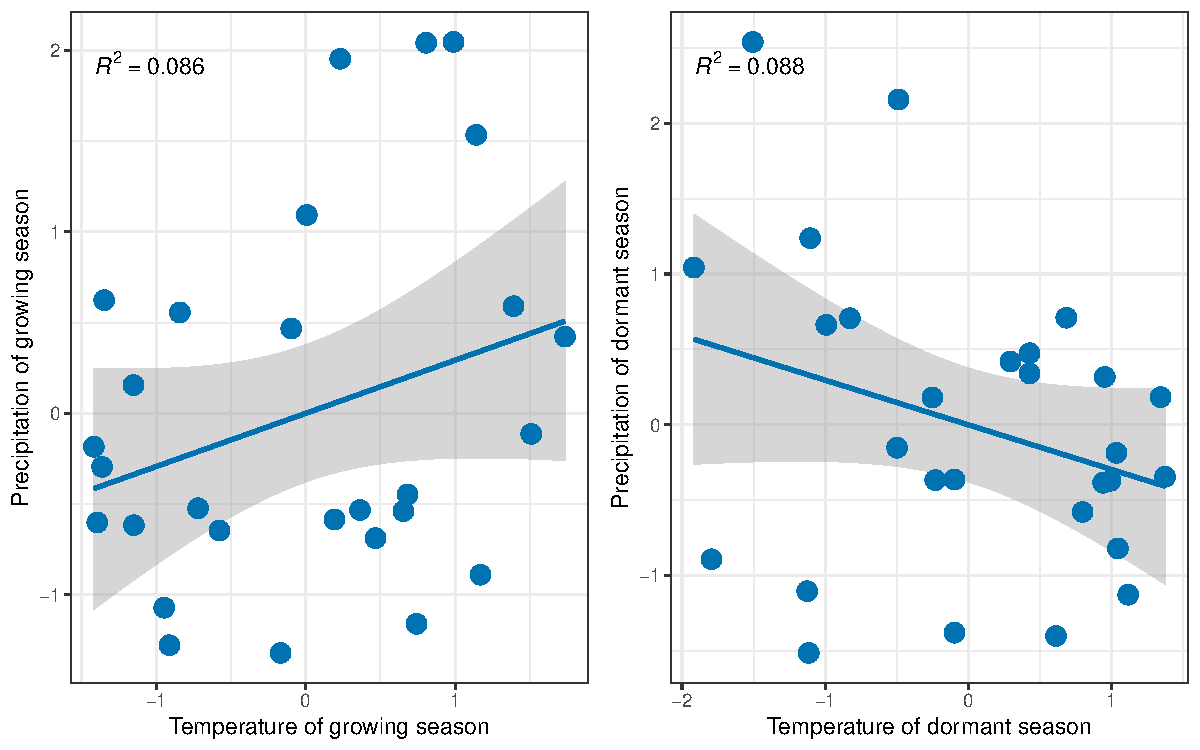
\includegraphics[width = \linewidth]{Varianceexplained.pdf}
		\caption{\textbf{Relation between precipitation and temperature for each season (growing and dormant).} $R^2$ indicates the value of proportion of explained variance between the temperature and precipitation}
	\end{figure}
	
  \begin{figure}[H]
		\centering
		\includegraphics[width = \linewidth]{PPC.pdf}
		\caption{\textbf{Consistency between real data and simulated values suggests that the fitted model accurately describes the data}. Graph shows density curves for the observed data (light blue ) along with the simulated values (dark blue). The first column shows the linear models and the second column shows the 2 degree polynomial models.}
	\end{figure}

\subsection*{Section S1}
\begin{subequations} 
	\begin{align}
		   S \sim Bernoulli(\hat{S}) \\
		   F \sim Bernoulli(\hat{F}) \\
		   G \sim Zero-truncated \ Poisson \ inverse\ Gaussian(\hat{G}) \\
		   Fer \sim Zero-truncated \ negative \ binomial(\hat{Fer}) 
    \end{align}
\end{subequations}
\begin{subequations} 
	\begin{align}
		   \hat{S} = \frac{exp (f(\mu))}{1 + exp (f(\mu))}  \\
		   \hat{F} = \frac{exp (f(\mu))}{1 + exp (f(\mu))}  \\
		   \textcolor{red}{\hat{G} = exp (f(\mu))} \\
		   \textcolor{red}{\hat{Fer} = exp (f(\mu))}
    \end{align}
\end{subequations}
\begin{equation} \label{eq:f_rate}
\begin{split}
f(\mu) = \beta_{0} + \beta_{1}size + \beta_{2}sex + \beta_{3}pptgrow + \beta_{4}pptdorm + \beta_{5}tempgrow\\ 
+ \beta_{6}tempdorm + \beta_{7}pptgrow*sex + \beta_{8}pptdorm*sex + \beta_{9}tempgrow*sex \\ 
+ \beta_{10}tempdorm*sex + \beta_{11}size*sex + \beta_{12}pptgrow*tempgrow\\
+ \beta_{13}pptdorm*tempdorm + \beta_{14}pptgrow*tempgrow*sex\\
+ \beta_{15}pptdorm*tempdorm*sex + \beta_{16}pptgrow^2 + \beta_{17}pptdorm^2 \\
+ \beta_{18}tempgrow^2 + \beta_{19}tempdorm^2 + \beta_{20}pptgrow^2*sex \\
+ \beta_{21}pptdorm^2*sex + \beta_{22}tempgrow^2*sex \\ 
+ \beta_{23}tempdorm^2*sex + \phi + \rho + \nu 
\end{split}
\end{equation}

\bibliographystyle{ecology}
\bibliography{Forecasting}
\end{document}
